\documentclass[aspectratio=169]{beamer}
\usetheme{default}
\setbeamertemplate{navigation symbols}{}
\setbeamertemplate{headline}{}

\usepackage{booktabs}
\usepackage{amsmath}
\usepackage{graphicx}
\usepackage{tikz}
\usetikzlibrary{calc}

\definecolor{deepInk}{HTML}{1B1F4A}
\definecolor{plumNight}{HTML}{5C2DA8}
\definecolor{candyPink}{HTML}{FF4FA8}
\definecolor{sunOrange}{HTML}{FFA640}
\definecolor{aquaPop}{HTML}{2ED6C5}
\definecolor{softSky}{HTML}{DDF0FF}
\definecolor{textInk}{HTML}{1F2644}

\setbeamercolor{normal text}{fg=textInk,bg=white}
\setbeamercolor{structure}{fg=plumNight}
\setbeamercolor{frametitle}{fg=white,bg=deepInk}
\setbeamercolor{itemize item}{fg=candyPink}
\setbeamercolor{itemize subitem}{fg=aquaPop}
\setbeamercolor{author in head/foot}{bg=deepInk,fg=white}
\setbeamercolor{date in head/foot}{bg=candyPink,fg=white}
\setbeamerfont{frametitle}{size=\large,series=\bfseries}

\setbeamertemplate{itemize item}{\color{candyPink}$\blacktriangleright$}
\setbeamertemplate{itemize subitem}{\color{aquaPop}$\bullet$}

\setbeamertemplate{background}{
\begin{tikzpicture}[remember picture,overlay]
  \path[shade, left color=softSky, right color=sunOrange!16]
    (current page.south west) rectangle (current page.north east);
  \fill[candyPink!18] ($(current page.north east)+(-0.9,-0.85)$) circle (1.15cm);
  \fill[aquaPop!20] ($(current page.south west)+(0.9,0.8)$) circle (1.2cm);
  \fill[sunOrange!35] ($(current page.south east)+(-0.55,0.55)$) circle (0.58cm);
\end{tikzpicture}
}

\setbeamertemplate{frametitle}{
  \begin{tikzpicture}[remember picture,overlay]
    \fill[deepInk!95,rounded corners=8pt]
      ([xshift=0.55cm,yshift=-0.2cm]current page.north west)
      rectangle
      ([xshift=-0.55cm,yshift=-1.1cm]current page.north east);
    \fill[candyPink] ([xshift=0.9cm,yshift=-0.5cm]current page.north west) circle (0.11cm);
    \fill[sunOrange] ([xshift=1.2cm,yshift=-0.5cm]current page.north west) circle (0.11cm);
    \fill[aquaPop] ([xshift=1.5cm,yshift=-0.5cm]current page.north west) circle (0.11cm);
    \node[anchor=west,text=white,font=\bfseries\large]
      at ([xshift=1.95cm,yshift=-0.65cm]current page.north west) {\insertframetitle};
  \end{tikzpicture}
  \vspace{0.94cm}
}

\setbeamertemplate{footline}[frame number]
\setbeamercolor{page number in head/foot}{fg=deepInk}

\title[ISA-TF Paper]{Metro Ridership Forecasting using Inter-Station-Aware Transformer Networks}
\subtitle{Big Data Course Presentation (10 minutes max)}
\author[Team of 4]{Nima DAVARI \and Maksym DOLHOV \and Khanh Bao ba \and Mehdi AGHAEI}
\institute[Big Data Course]{Big Data Course}
\date{\today}

\begin{document}

\begin{frame}[plain]
  
\begin{tikzpicture}[remember picture,overlay]
    \path[shade, left color=deepInk, right color=plumNight]
      (current page.south west) rectangle (current page.north east);
  \end{tikzpicture}

  \vspace*{0.25cm}
  \begin{flushright}
    
\includegraphics[width=0.34\linewidth]{images/paris_cite_logo_white.png}
  \end{flushright}

  \vspace{0.95cm}
  {\usebeamerfont{title}\color{white}\inserttitle\par}
  \vspace{0.42cm}
  {\usebeamerfont{subtitle}\color{sunOrange}\insertsubtitle\par}
  \vspace{1.0cm}
  {\usebeamerfont{author}\color{white}\insertauthor\par}
  \vspace{0.18cm}
  {\usebeamerfont{institute}\color{white}\insertinstitute\par}
\end{frame}

% ------------------------- Presenter 1 -------------------------
\section{Presenter 1}

\begin{frame}{[1/12] Problem Context (Presenter 1)}
  \begin{itemize}
    \item Metro systems need station-level inflow/outflow forecasts for operations.
    \item Better forecasting improves train scheduling, staffing, maintenance, and capacity planning.
    \item Wrong forecasts can increase congestion and reduce service quality.
    \item The task is hard because demand is both \textbf{temporal} and \textbf{network-dependent}.
  \end{itemize}
\end{frame}

\begin{frame}{[2/12] Research Gap and Paper Idea (Presenter 1)}
  \begin{itemize}
    \item Prior methods include statistical, machine learning, and hybrid approaches.
    \item Many RNN/GCN-based methods are strong for short horizon but can degrade for longer horizon.
    \item This paper proposes \textbf{ISA-TF}: a unified transformer framework for metro ridership forecasting.
    \item Core idea: fuse ridership history with inter-station topology information.
  \end{itemize}
\end{frame}

\begin{frame}{[3/12] Claimed Contributions (Presenter 1)}
  \begin{itemize}
    \item New \textbf{Inter-Station-Aware Transformer Networks} architecture.
    \item Uses three metro graph views: physical, semantic similarity, and correlation.
    \item Evaluated on SHMetro and HZMetro benchmarks.
    \item Reports stronger long-horizon performance and much lower parameter count.
  \end{itemize}
\end{frame}

% ------------------------- Presenter 2 -------------------------
\section{Presenter 2}

\begin{frame}{[4/12] Problem Formulation (Presenter 2)}
  \begin{itemize}
    \item Input: past ridership sequence and metro graph:
    \[
      \{D^N_{t-n+1}, \dots, D^N_t\},\; G
      \rightarrow
      \{\hat{D}^N_{t+1}, \dots, \hat{D}^N_{t+m}\}
    \]
    \item Each station signal contains two values: inflow and outflow.
    \item In experiments: \(n=4\) past intervals (60 min total), \(m=4\) future intervals.
    \item Inference is autoregressive, so horizons longer than 60 min are possible.
  \end{itemize}
\end{frame}

\begin{frame}{[5/12] Metro Graph Representation (Presenter 2)}
  \begin{columns}[T,totalwidth=\textwidth]
    \column{0.49\textwidth}
      \centering
      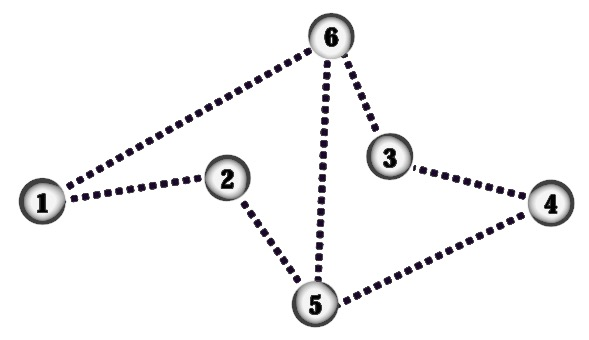
\includegraphics[width=\linewidth]{images/interstation_graph_physical.jpg}\\
      \scriptsize Physical topology view
    \column{0.49\textwidth}
      \centering
      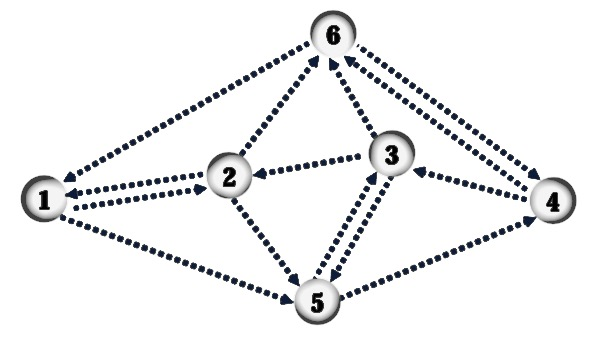
\includegraphics[width=\linewidth]{images/interstation_graph_enhanced.jpg}\\
      \scriptsize Enhanced inter-station relation view
  \end{columns}
  \vspace{0.35em}
  \small
  \textbf{Explanation:} The paper represents the metro network with complementary graph structures, not only direct neighboring links. This helps the model capture both local structure and richer cross-station interaction patterns, which improves forecasting robustness when passenger flow dependencies are not purely geographic.
\end{frame}

\begin{frame}{[6/12] ISA-TF Architecture (Presenter 2)}
  \begin{itemize}
    \item Encoder-decoder transformer backbone with positional encoding.
    \item Encoder processes historical ridership tokens.
    \item Intermediate fusion concatenates encoder output with \(M_p, M_s, M_c\), then feed-forward layer.
    \item Decoder uses self-attention and cross-attention to generate future ridership autoregressively.
  \end{itemize}
\end{frame}

% ------------------------- Presenter 3 -------------------------
\section{Presenter 3}

\begin{frame}{[7/12] Datasets (Presenter 3)}
  \begin{table}
    \centering
    \small
    \begin{tabular}{lll}
      \toprule
      Property & SHMetro & HZMetro \\
      \midrule
      Period & Jul--Sep 2016 & Jan 1--25, 2019 \\
      Stations & 288 & 80 \\
      Physical edges & 958 & 248 \\
      Avg daily passengers & 8.82M & 2.35M \\
      Interval & 15 minutes & 15 minutes \\
      \bottomrule
    \end{tabular}
  \end{table}
  \vspace{0.2em}
  \small SHMetro has 811.8M recorded transactions.
\end{frame}

\begin{frame}{[8/12] Experimental Setup (Presenter 3)}
  \begin{itemize}
    \item Preprocessing creates the three graph types per dataset.
    \item Training details: Adam optimizer, 250 epochs, \(L_2\) loss.
    \item Model hyperparameters: embedding size 512, 8 attention heads.
    \item Evaluation metrics: RMSE and MAE.
    \item Baselines: HM, GB, MLP, RNN-GRU, STG2Seq, DCRNN, PVCGN.
  \end{itemize}
\end{frame}

\begin{frame}{[9/12] Main Results (Presenter 3)}
  \small
  \begin{table}
    \centering
    \begin{tabular}{llll}
      \toprule
      Dataset & Horizon & ISA-TF (RMSE/MAE) & PVCGN (RMSE/MAE) \\
      \midrule
      SHMetro & 60 min & \textbf{48.43/23.87} & 55.27/26.29 \\
      HZMetro & 60 min & \textbf{41.68/24.91} & 42.61/24.93 \\
      SHMetro & 15 min & 45.85/\textbf{23.05} & \textbf{44.97}/23.29 \\
      \bottomrule
    \end{tabular}
  \end{table}
  \vspace{0.3em}
  \begin{itemize}
    \item Strong long-horizon robustness is the key result.
    \item Short horizon remains competitive with the prior SOTA.
  \end{itemize}
\end{frame}

% ------------------------- Presenter 4 -------------------------
\section{Presenter 4}

\begin{frame}{[10/12] Efficiency Comparison (Presenter 4)}
  \begin{columns}[T,totalwidth=\textwidth]
    \column{0.56\textwidth}
      \centering
      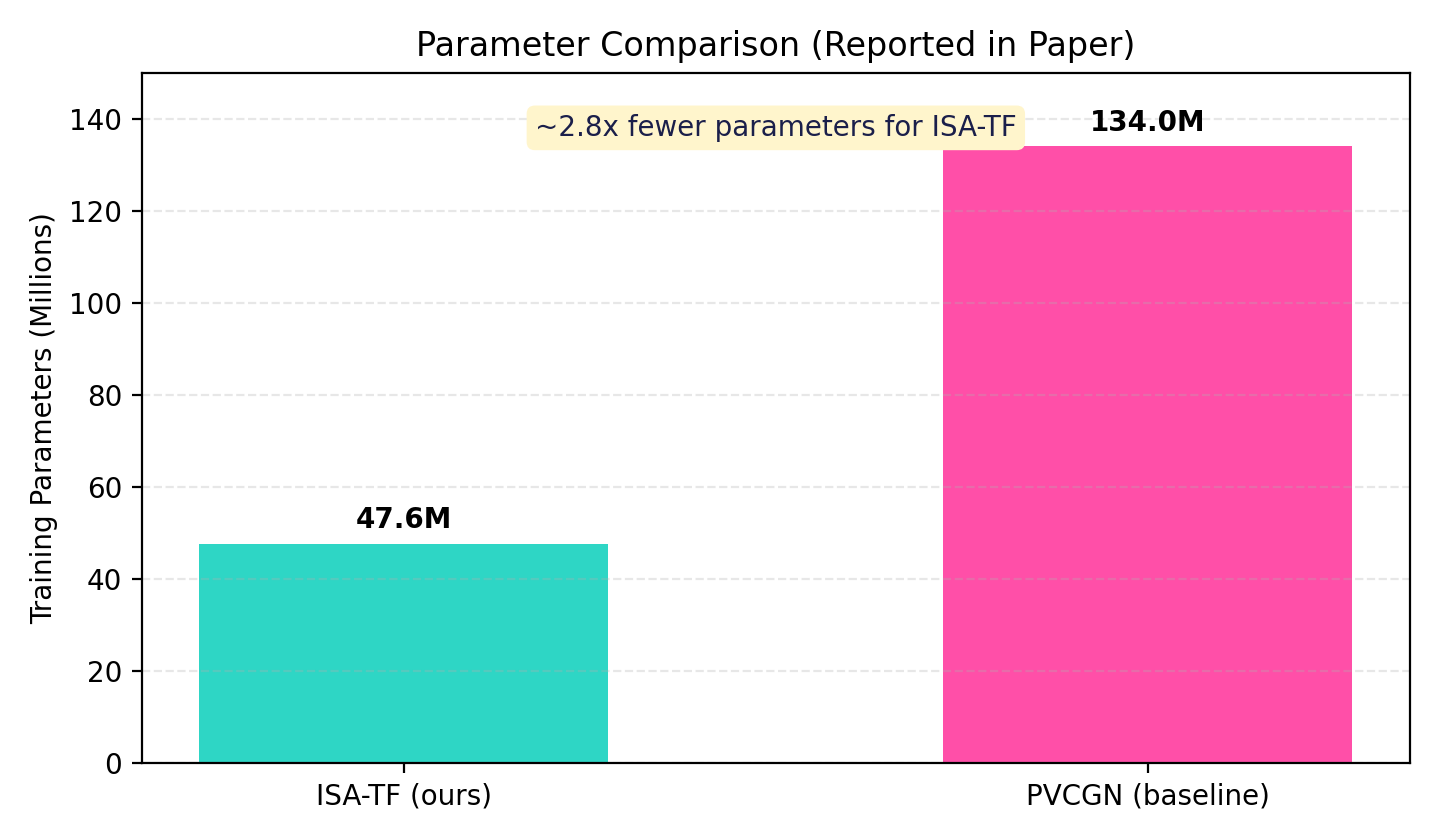
\includegraphics[width=\linewidth]{images/parameter_efficiency_chart.png}
    \column{0.42\textwidth}
      \small
      \textbf{Explanation:} Based on the paper's reported values, ISA-TF uses 47.6M parameters while PVCGN requires about 134M. This means ISA-TF is around 2.8x lighter, which is important for faster training, lower memory use, and easier deployment while keeping competitive or better forecasting performance.
  \end{columns}
  \vspace{0.3em}
  \footnotesize Source: values reported by the paper (Figure 2 discussion and results section).
\end{frame}

\begin{frame}{[11/12] Discussion for Class (Presenter 4)}
  \begin{itemize}
    \item \textbf{Strengths:} unified architecture, good long-horizon behavior, parameter efficiency.
    \item \textbf{Caveat:} evaluation is on two datasets only; generalization should be tested further.
    \item \textbf{Possible extensions:}
    \begin{itemize}
      \item Include weather/events/holidays as exogenous features.
      \item Add uncertainty intervals, not only point forecasts.
      \item Evaluate transfer across cities with different network shapes.
    \end{itemize}
  \end{itemize}
\end{frame}

\begin{frame}{[12/12] Conclusion and Q\&A (Presenter 4)}
  \begin{itemize}
    \item ISA-TF combines ridership history with topology-aware graph information.
    \item It matches or beats prior methods, especially for 45--60 minute horizons.
    \item It achieves this with about 3x fewer parameters than PVCGN.
  \end{itemize}
  \vspace{0.6em}
  \textbf{Takeaway:} topology-aware transformers are a strong option for scalable metro ridership forecasting.
  \vspace{0.8em}

  \small Reference: K. Saleh, A.-S. Mihaita, and Y. Ou, 2023 IEEE ITSC (Manuscript 470 preprint).
\end{frame}

\end{document}
